%
\section{Introduction}
\label{sec:intro}


\cxj{Is your goal reconstruction or building extraction? The introduction should explain the overall goal. What are the challenges for building modeling from remote sensing images? What kind of work has been done in the literature? Why do we focus on building detection? What are our contributions?}

\IEEEPARstart{B}{uilding} extraction, which aims to extract rooftop\footnote{Because the data sets used in our article are high altitude remote sensing images which could be considered as the top views of the ground. Therefore, we do not distinguish the concepts of buildings and rooftops in the subsequent description.} in a large-scale remote sensing image, remains one of the main challenges have been studied for decades in the field of remote sensing. Moreover, automatic extraction of building rooftops from aerial and satellite imagery is an important step in many applications, such as: urban planing, automated map making, 3D city modeling, updating geographical dataset and military reconnaissance. It is particularly difficult to extract rooftop from remote sensing images at the pixel level because of the following three reasons: \romannumeral1) Density of the structures in the scene. A rural scene has low density but an urban scene has high density, with a suburban scene in between (medium density).  \romannumeral2) Shape of the structure. Buildings come in many shapes from simple rectangular blocks with flat roof to complex shapes with intricate, multi-based roof structure.  \romannumeral3) Image quality. Images vary in terms of contrast, resolution, and visibility  \cite{IEEEexample:huertas1988detecting}. Some remote sensing patches are shown in Fig.~\ref{fig:intro} \cxj{do not use the figure no directly. using ref{}..} , which illustrate the challenges of building extraction task.


\begin{figure}
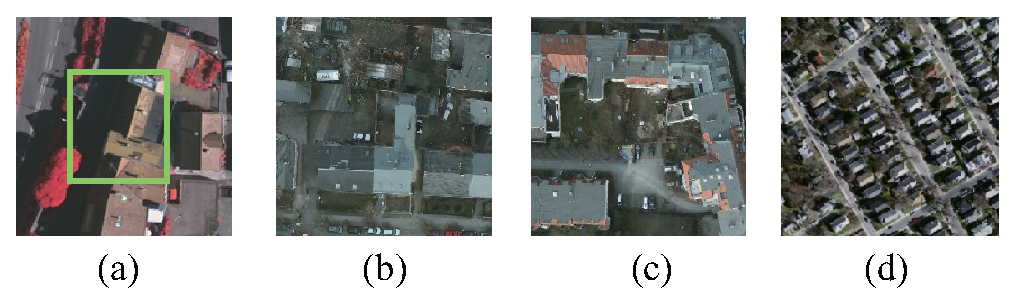
\includegraphics[width=8.7cm]{Figures/challenge.eps}
\caption{Examples of remote sensing patches with different kinds of challenges. (a) Shadow occlusion in green frame. (b) Low inter-class differences. (c) High intra class variance. (d) A lot of tiny buildings close to each other.}
\label{fig:intro}
\end{figure}


In the past decades, many researchers made some experimental investigations to extract buildings automatically. In the early days, many knowledge-based methods were put forward by \cite{IEEEexample:huertas1988detecting}, \cite{IEEEexample:noronha2001detection}, \cite{IEEEexample:nosrati2009novel}, \cite{IEEEexample:izadi2012three}, \cite{IEEEexample:wang2015efficient} whose basic ideas are derived from prior knowledge of buildings, for instance, buildings are closed polygons made up of some straight lines. Some others are energy based methods which mainly includes the variational level set evolution, improved snake model and graph cut \cite{IEEEexample:cote2013automatic}, \cite{IEEEexample:peng2005improved}, \cite{IEEEexample:sirmacek2009urban}.


In recent years, with the development of machine learning, many machine-learning techniques are gradually penetrating into the remote sensing domain.
At first, some shallow networks were proposed for multiple object extraction\cite{IEEEexample:mnih2013machine}, \cite{IEEEexample:saito2016multiple}, \cite{IEEEexample:alshehhi2017simultaneous},\cite{IEEEexample:zhao2017contextually}. Afterwards, with increasing computer power, deep learning developed rapidly and introduced into the field of remote sensing. At the same time, some researchers tried Convolutional Neural Networks (CNNs) for aerial images classification and semantic pixel labelling~\cite{IEEEexample:paisitkriangkrai2015effective}, \cite{IEEEexample:liu2017dense}, \cite{IEEEexample:audebert2017deep}, \cite{IEEEexample:kampffmeyer2017urban}, \cite{IEEEexample:he2017multi}.


In this work, a relatively simple, but very effective, manner is proposed and combined into a general CNN architecture for building extraction. We take full advantages of the low-level appearance information as well as high-level semantic information by the novel fusion operation in a way of stage by stage.
Numerous experiments conducted on three remote sensing image datasets all obtain fairly good results.
We further extend our work to the field of 3D modeling as the part of building detection. And it be easily intergrated into the pipeline of building reconstruction.
Our technical contributions are:
%
\begin{enumerate}
	\item A effective hierarchical fusion operation which is specially designed for multi-scale building extraction is proposed. Combining with a trimmed VGG16 Net, a novel network is presented, named HF-FCN that can deal with the problems of different sizes, diverse appearance and mutual occlusion of buildings and etc.
	\item HF-FCN is an end-to-end network that does not need any post processing. And the approach is significantly computationally efficient than existing techniques. Besides, the overall accuracy based on HF-FCN exceeds the state-of-art algorithms.
	\item A extend exploration for building reconstruction of large-scale urban areas is studied. And the experiments reveal the method well preserve buildings details.
\end{enumerate}

The remainder of this paper is organized as follows. Sec.~\ref{Sec:RelatedWork} sums up the related works in the past.
In Sec.~\ref{Sec:HF-FCN}, we introduce the fusion operation and architecture of HF-FCN. The training steps are also presented.
And in Sec.~\ref{Sec:exp}, a brief description of the dataset used for our task is provided. HF-FCN training strategies, details and its evaluation metrics are also described.
In Sec.~\ref{Sec:Res},we display and analysis the experimental results.
Extension in 3D building modeling are presented in Sec.~\ref{sec:app}.
Finally, the conclusion is discussed in Sec.~\ref{Sec:Con}.
